\label{chap:implementation}

\epigraph{Python is the "most powerful language you can still read".}{\textit{Paul Dubois}}

\section{FANUC robots programming specifics and FANUC software}

\subsection{FANUC Roboguide}

FANUC Roboguide is a proprietary robot simulator and offline programming tool developed by FANUC. Roboguide is in many ways similar to RoboDK.  Like RoboDK, it supports the creation of robot stations, importing of CAD files and CAD-to-path features. The main difference is that Roboguide is limited to FANUC robots and FANUC related technology and procedures. In contrast, RoboDK is not limited to one robot manufactures and is universal and expandable. Roboguide is used for this project to compile the created FANUC programs and upload them to the FANUC robot controller. Roboguide offers several Simulation Software Options tailored for specific robotic arm applications:

\begin{itemize}

\item FANUC Roboguide HandlingPRO - simulating material handling applications including load/unload, packaging, assembly and material removal
\item FANUC Roboguide PaintPRO - simulating painting applications
\item FANUC Roboguide WeldPRO - simulating robotic arc welding process
\item FANUC Roboguide PalletPRO and PalletTool - simulating palletizing applications

\end{itemize}

An example of a Roboguide station is shown in Figure \ref{fig:roboguide}. The version of FANUC Roboguide used for this project is 8.30104.00.35 (Rev. K). 

\begin{figure}[h]
    \centering
    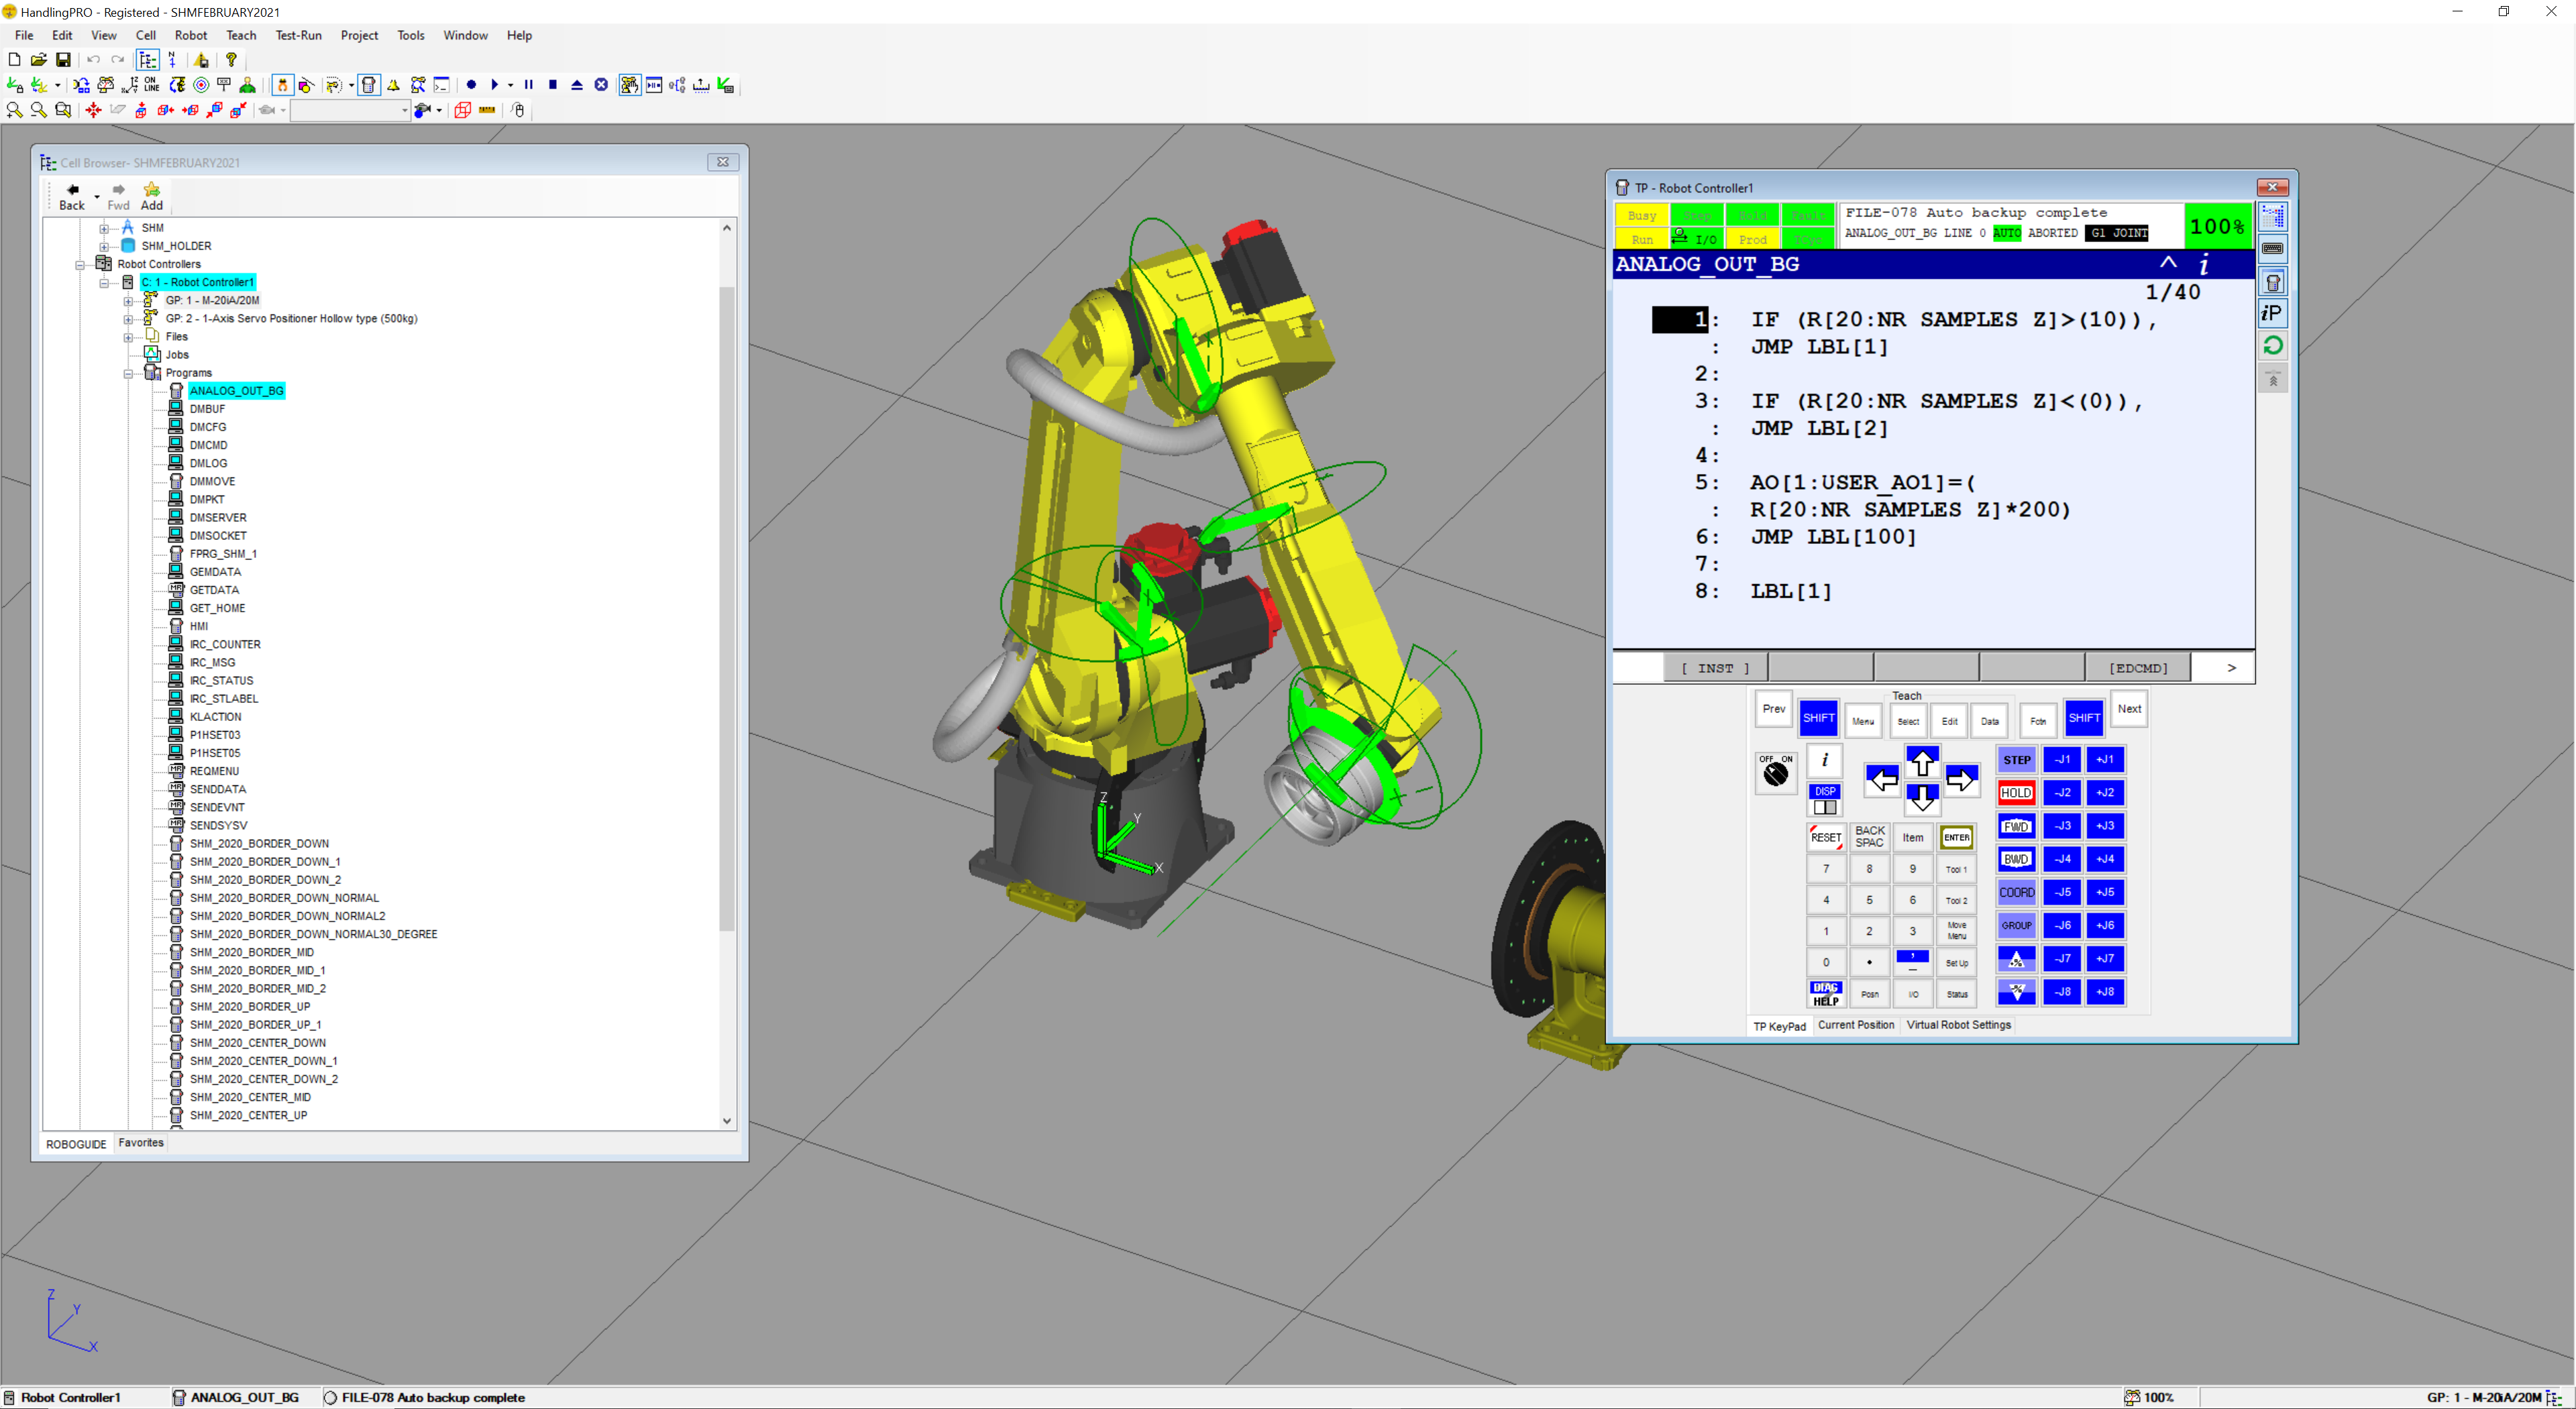
\includegraphics[width=0.9\linewidth]{img/roboguide.PNG}
    \caption{FANUC Roboguide work cell - user interface example.}
    \label{fig:roboguide}
\end{figure}

\subsection{FANUC robots programming languages}

The FANUC company implements two programming languages for programming their robot controllers: Teach Pendant (TP) or KAREL. The Teach Pendant language is mainly used for motion control of the robotic arm and edited via the Pendant. Teach pendant programs are either binary files (\mintinline{shell-session}{.tp} file extension) or can be human-readable ASCII files (\mintinline{shell-session}{.ls} file extension). The KAREL language is a high-level language and does not support robot movements. KAREL is mainly used to implement algorithms. KAREL programs can be only edited using a Personal Computer, and they can not be edited using a Pendant.

\subsection{Compiling a FANUC TP program}

Only a Teach Pendant program in binary format can be run on FANUC controllers. Because RoboDK creates TP programs as human-readable ASCII files, the Teach Pendant programs need to be converted to binary format before uploading them to the robot controller. Two options to convert .ls programs to .tp programs exist:

\begin{enumerate}
\item The ASCII Upload option must be loaded on the robot controller. After upload an (\mintinline{shell-session}{.ls} file to the controller it is automatically converted to a (\mintinline{shell-session}{.tp} file.
\item The program is compiled and uploaded either using the WinOLPC  tools via Roboguide or using the WinOLPC tools directly

\end{enumerate}

\section{Robot machining projects in RoboDK}

The applications of robot machining in the industry are numerous. Some applications include:

\begin{itemize}

    \item milling
    \item drilling
    \item chamfering
    \item deburring

\end{itemize}

RoboDK offers three types of robot manufacturing projects:

\begin{itemize}

    \item Robot machining project
    \item Curve follow project 
    \item Point follow project 

\end{itemize}

This chapter deals with setting up a Curve follow project in RoboDK. In laser shock peening, the laser (the tool) is static, and the robot holds the object. Therefore, a Curve follow project with a constant tool orientation is set up in RoboDK.

\subsection{Setting up a Curve follow project in RoboDK}


\section{RoboDK API for Python}

\section{Installation, Python setup and path settings of RoboDK API}

\section{Modifying a post processor}


